\documentclass[twoside]{book}

% Packages required by doxygen
\usepackage{fixltx2e}
\usepackage{calc}
\usepackage{doxygen}
\usepackage{graphicx}
\usepackage[utf8]{inputenc}
\usepackage{makeidx}
\usepackage{multicol}
\usepackage{multirow}
\PassOptionsToPackage{warn}{textcomp}
\usepackage{textcomp}
\usepackage[nointegrals]{wasysym}
\usepackage[table]{xcolor}

% Font selection
\usepackage[T1]{fontenc}
\usepackage{mathptmx}
\usepackage[scaled=.90]{helvet}
\usepackage{courier}
\usepackage{amssymb}
\usepackage{sectsty}
\renewcommand{\familydefault}{\sfdefault}
\allsectionsfont{%
  \fontseries{bc}\selectfont%
  \color{darkgray}%
}
\renewcommand{\DoxyLabelFont}{%
  \fontseries{bc}\selectfont%
  \color{darkgray}%
}
\newcommand{\+}{\discretionary{\mbox{\scriptsize$\hookleftarrow$}}{}{}}

% Page & text layout
\usepackage{geometry}
\geometry{%
  a4paper,%
  top=2.5cm,%
  bottom=2.5cm,%
  left=2.5cm,%
  right=2.5cm%
}
\tolerance=750
\hfuzz=15pt
\hbadness=750
\setlength{\emergencystretch}{15pt}
\setlength{\parindent}{0cm}
\setlength{\parskip}{0.2cm}
\makeatletter
\renewcommand{\paragraph}{%
  \@startsection{paragraph}{4}{0ex}{-1.0ex}{1.0ex}{%
    \normalfont\normalsize\bfseries\SS@parafont%
  }%
}
\renewcommand{\subparagraph}{%
  \@startsection{subparagraph}{5}{0ex}{-1.0ex}{1.0ex}{%
    \normalfont\normalsize\bfseries\SS@subparafont%
  }%
}
\makeatother

% Headers & footers
\usepackage{fancyhdr}
\pagestyle{fancyplain}
\fancyhead[LE]{\fancyplain{}{\bfseries\thepage}}
\fancyhead[CE]{\fancyplain{}{}}
\fancyhead[RE]{\fancyplain{}{\bfseries\leftmark}}
\fancyhead[LO]{\fancyplain{}{\bfseries\rightmark}}
\fancyhead[CO]{\fancyplain{}{}}
\fancyhead[RO]{\fancyplain{}{\bfseries\thepage}}
\fancyfoot[LE]{\fancyplain{}{}}
\fancyfoot[CE]{\fancyplain{}{}}
\fancyfoot[RE]{\fancyplain{}{\bfseries\scriptsize Generated on Sun May 24 2015 21\+:38\+:55 for N\+F\+Q by Doxygen }}
\fancyfoot[LO]{\fancyplain{}{\bfseries\scriptsize Generated on Sun May 24 2015 21\+:38\+:55 for N\+F\+Q by Doxygen }}
\fancyfoot[CO]{\fancyplain{}{}}
\fancyfoot[RO]{\fancyplain{}{}}
\renewcommand{\footrulewidth}{0.4pt}
\renewcommand{\chaptermark}[1]{%
  \markboth{#1}{}%
}
\renewcommand{\sectionmark}[1]{%
  \markright{\thesection\ #1}%
}

% Indices & bibliography
\usepackage{natbib}
\usepackage[titles]{tocloft}
\setcounter{tocdepth}{3}
\setcounter{secnumdepth}{5}
\makeindex

% Custom commands
\newcommand{\clearemptydoublepage}{%
  \newpage{\pagestyle{empty}\cleardoublepage}%
}


%===== C O N T E N T S =====

\begin{document}

% Titlepage & ToC
\pagenumbering{roman}
\begin{titlepage}
\vspace*{7cm}
\begin{center}%
{\Large N\+F\+Q \\[1ex]\large 1.\+0 }\\
\vspace*{1cm}
{\large Generated by Doxygen 1.8.8}\\
\vspace*{0.5cm}
{\small Sun May 24 2015 21:38:55}\\
\end{center}
\end{titlepage}
\clearemptydoublepage
\tableofcontents
\clearemptydoublepage
\pagenumbering{arabic}

%--- Begin generated contents ---
\chapter{Hierarchical Index}
\section{Class Hierarchy}
This inheritance list is sorted roughly, but not completely, alphabetically\+:\begin{DoxyCompactList}
\item \contentsline{section}{Agent}{\pageref{a00001}}{}
\begin{DoxyCompactList}
\item \contentsline{section}{Nao\+Agent}{\pageref{a00003}}{}
\end{DoxyCompactList}
\item \contentsline{section}{Main\+Handler}{\pageref{a00002}}{}
\item \contentsline{section}{N\+F\+Q}{\pageref{a00004}}{}
\item \contentsline{section}{Task}{\pageref{a00006}}{}
\begin{DoxyCompactList}
\item \contentsline{section}{Predator\+Prey\+Task}{\pageref{a00005}}{}
\end{DoxyCompactList}
\item \contentsline{section}{W\+S\+Handler}{\pageref{a00007}}{}
\end{DoxyCompactList}

\chapter{Class Index}
\section{Data Structures}
Here are the data structures with brief descriptions\+:\begin{DoxyCompactList}
\item\contentsline{section}{{\bf ann\+\_\+t} \\*Struct representing a neural network }{\pageref{structann__t}}{}
\end{DoxyCompactList}

\chapter{Class Documentation}
\section{Agent Class Reference}
\label{a00001}\index{Agent@{Agent}}


Provides a default interface for \doxyref{Agent}{p.}{a00001} class.  


Inheritance diagram for Agent\+:\begin{figure}[H]
\begin{center}
\leavevmode
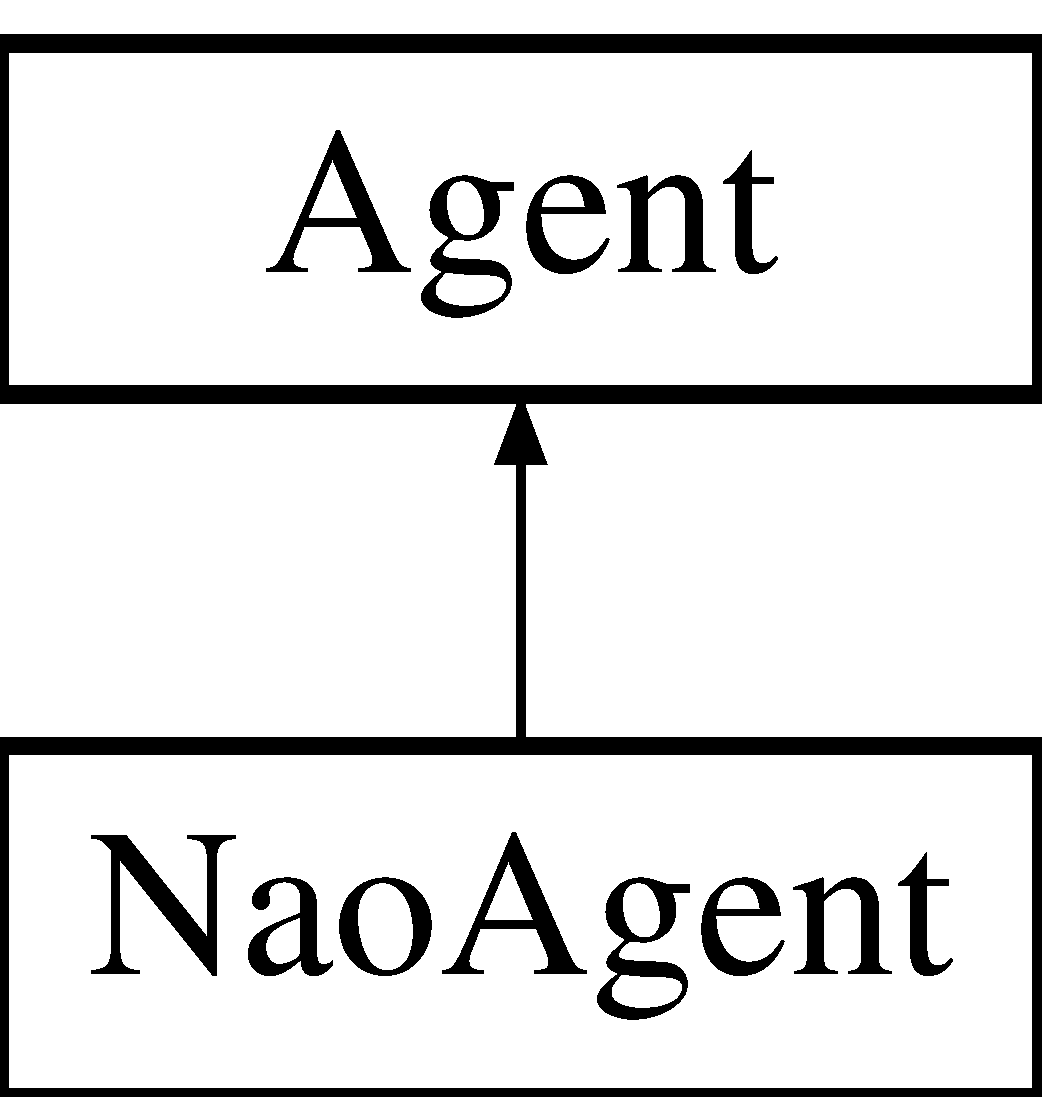
\includegraphics[height=2.000000cm]{a00001}
\end{center}
\end{figure}
\subsection*{Public Member Functions}
\begin{DoxyCompactItemize}
\item 
def {\bf connect}
\begin{DoxyCompactList}\small\item\em This method should handle connection to a real world agent. \end{DoxyCompactList}\item 
def {\bf disconnect}
\begin{DoxyCompactList}\small\item\em This methods should handle disconnection from a real world agent. \end{DoxyCompactList}\item 
def {\bf do}
\begin{DoxyCompactList}\small\item\em This methods handles performing selected action according to action number on a real world agent. \end{DoxyCompactList}\end{DoxyCompactItemize}


\subsection{Detailed Description}
Provides a default interface for \doxyref{Agent}{p.}{a00001} class. 

\subsection{Member Function Documentation}
\index{Agent\+::\+Agent@{Agent\+::\+Agent}!connect@{connect}}
\index{connect@{connect}!Agent\+::\+Agent@{Agent\+::\+Agent}}
\subsubsection[{connect}]{\setlength{\rightskip}{0pt plus 5cm}def connect (
\begin{DoxyParamCaption}
\item[{}]{self}
\end{DoxyParamCaption}
)}\label{a00001_a0f3e881a92d7a1b4d6d07d9e63180c98}


This method should handle connection to a real world agent. 

This method must be implemented \index{Agent\+::\+Agent@{Agent\+::\+Agent}!disconnect@{disconnect}}
\index{disconnect@{disconnect}!Agent\+::\+Agent@{Agent\+::\+Agent}}
\subsubsection[{disconnect}]{\setlength{\rightskip}{0pt plus 5cm}def disconnect (
\begin{DoxyParamCaption}
\item[{}]{self}
\end{DoxyParamCaption}
)}\label{a00001_afab97b4023d6e30d95344406b3655983}


This methods should handle disconnection from a real world agent. 

This method must be implemented \index{Agent\+::\+Agent@{Agent\+::\+Agent}!do@{do}}
\index{do@{do}!Agent\+::\+Agent@{Agent\+::\+Agent}}
\subsubsection[{do}]{\setlength{\rightskip}{0pt plus 5cm}def do (
\begin{DoxyParamCaption}
\item[{}]{self, }
\item[{}]{action\+\_\+number}
\end{DoxyParamCaption}
)}\label{a00001_a412db3f49e4869fa4cb87535dcc77caf}


This methods handles performing selected action according to action number on a real world agent. 

This method must be implemented 
\begin{DoxyParams}{Parameters}
{\em action\+\_\+number} & Number of action to be performed \\
\hline
\end{DoxyParams}

\section{Main\+Handler Class Reference}
\label{a00002}\index{Main\+Handler@{Main\+Handler}}


Operates a web server for web application.  




Inherits Request\+Handler.

\subsection*{Public Member Functions}
\begin{DoxyCompactItemize}
\item 
def {\bf get}
\begin{DoxyCompactList}\small\item\em Handles asynchronous web request and renders a web app. \end{DoxyCompactList}\end{DoxyCompactItemize}


\subsection{Detailed Description}
Operates a web server for web application. 

\subsection{Member Function Documentation}
\index{server\+::\+Main\+Handler@{server\+::\+Main\+Handler}!get@{get}}
\index{get@{get}!server\+::\+Main\+Handler@{server\+::\+Main\+Handler}}
\subsubsection[{get}]{\setlength{\rightskip}{0pt plus 5cm}def get (
\begin{DoxyParamCaption}
\item[{}]{request}
\end{DoxyParamCaption}
)}\label{a00002_a444a1328efb32d5d9d2dcb2efe855d3b}


Handles asynchronous web request and renders a web app. 


\begin{DoxyParams}{Parameters}
{\em request} & Web request received \\
\hline
\end{DoxyParams}

\section{Nao\+Agent Class Reference}
\label{a00003}\index{Nao\+Agent@{Nao\+Agent}}


Implementation of Agent interface on Nao robot in Webots simulator.  


Inheritance diagram for Nao\+Agent\+:\begin{figure}[H]
\begin{center}
\leavevmode
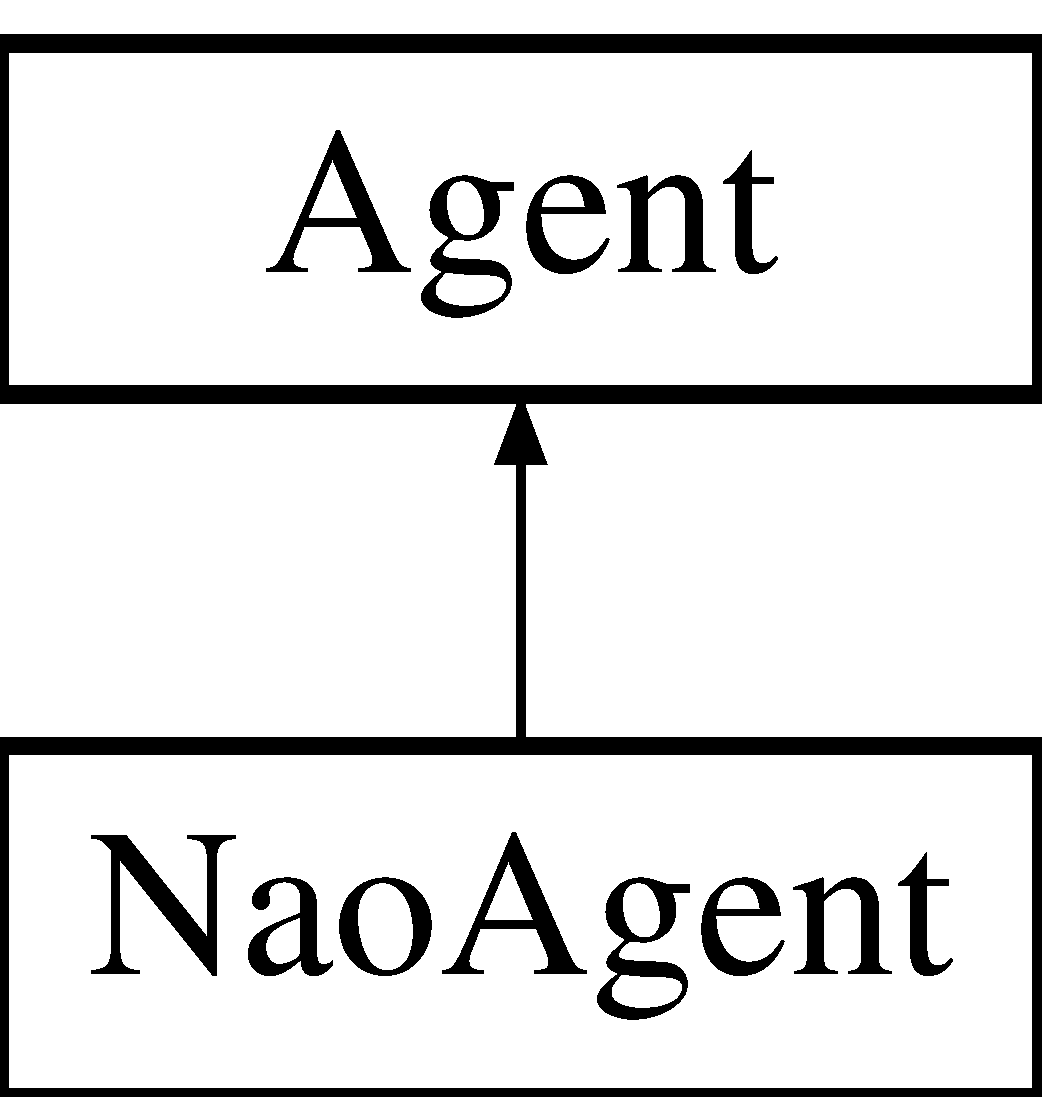
\includegraphics[height=2.000000cm]{a00003}
\end{center}
\end{figure}
\subsection*{Public Member Functions}
\begin{DoxyCompactItemize}
\item 
def {\bf \+\_\+\+\_\+init\+\_\+\+\_\+}\label{a00003_ac775ee34451fdfa742b318538164070e}

\begin{DoxyCompactList}\small\item\em Constructor method setups default parameters. \end{DoxyCompactList}\item 
def {\bf connect}
\begin{DoxyCompactList}\small\item\em Method handles connection to simulated robot and initialization of its features. \end{DoxyCompactList}\item 
def {\bf disconnect}\label{a00003_afab97b4023d6e30d95344406b3655983}

\begin{DoxyCompactList}\small\item\em Disconnects from simulated Nao. \end{DoxyCompactList}\item 
def {\bf do}
\begin{DoxyCompactList}\small\item\em Perform specified action from the set of all available motions. \end{DoxyCompactList}\item 
def {\bf go\+\_\+forward}\label{a00003_a74f88e9c727035ad050d4a1b5e16eb5f}

\begin{DoxyCompactList}\small\item\em This method performs movements along the X-\/axis, with 0.\+25m distance. \end{DoxyCompactList}\item 
def {\bf go\+\_\+right}\label{a00003_a1825cf4236b693f347db9c793206049c}

\begin{DoxyCompactList}\small\item\em This method performs a rotation 30 degrees to the right. \end{DoxyCompactList}\item 
def {\bf go\+\_\+left}\label{a00003_a3661eec663302a3b67351833c2c9b8de}

\begin{DoxyCompactList}\small\item\em This method perform movement 30 degrees left. \end{DoxyCompactList}\item 
def {\bf Stiffness\+On}
\begin{DoxyCompactList}\small\item\em Sets the stiffnes of Nao's joints to maximal value, to make him ready to perform motions. \end{DoxyCompactList}\end{DoxyCompactItemize}
\subsection*{Public Attributes}
\begin{DoxyCompactItemize}
\item 
{\bf robot\+\_\+ip}\label{a00003_a70221305bf8db6392330ef28121efd25}

\begin{DoxyCompactList}\small\item\em Default connection I\+P address. \end{DoxyCompactList}\item 
{\bf robot\+\_\+port}\label{a00003_a9282cdfa59976fe1cfc1a539df185c27}

\begin{DoxyCompactList}\small\item\em Default connection port. \end{DoxyCompactList}\end{DoxyCompactItemize}


\subsection{Detailed Description}
Implementation of Agent interface on Nao robot in Webots simulator. 

\subsection{Member Function Documentation}
\index{Nao\+Agent\+::\+Nao\+Agent@{Nao\+Agent\+::\+Nao\+Agent}!connect@{connect}}
\index{connect@{connect}!Nao\+Agent\+::\+Nao\+Agent@{Nao\+Agent\+::\+Nao\+Agent}}
\subsubsection[{connect}]{\setlength{\rightskip}{0pt plus 5cm}def connect (
\begin{DoxyParamCaption}
\item[{}]{self, }
\item[{}]{ip = {\ttfamily None}, }
\item[{}]{port = {\ttfamily None}}
\end{DoxyParamCaption}
)}\label{a00003_a0f3e881a92d7a1b4d6d07d9e63180c98}


Method handles connection to simulated robot and initialization of its features. 

It connection to the robot on specified Ip\+:port and initializes the robot to the init position, preparing it for motions. 
\begin{DoxyParams}{Parameters}
{\em ip} & I\+P address of a robot \\
\hline
{\em port} & Port number of a robot \\
\hline
\end{DoxyParams}
\begin{DoxyReturn}{Returns}
True, if connection was succesful, else False 
\end{DoxyReturn}
\index{Nao\+Agent\+::\+Nao\+Agent@{Nao\+Agent\+::\+Nao\+Agent}!do@{do}}
\index{do@{do}!Nao\+Agent\+::\+Nao\+Agent@{Nao\+Agent\+::\+Nao\+Agent}}
\subsubsection[{do}]{\setlength{\rightskip}{0pt plus 5cm}def do (
\begin{DoxyParamCaption}
\item[{}]{self, }
\item[{}]{action\+\_\+number}
\end{DoxyParamCaption}
)}\label{a00003_a412db3f49e4869fa4cb87535dcc77caf}


Perform specified action from the set of all available motions. 


\begin{DoxyParams}{Parameters}
{\em action\+\_\+number} & specifies position of action in the action list \\
\hline
\end{DoxyParams}
\index{Nao\+Agent\+::\+Nao\+Agent@{Nao\+Agent\+::\+Nao\+Agent}!Stiffness\+On@{Stiffness\+On}}
\index{Stiffness\+On@{Stiffness\+On}!Nao\+Agent\+::\+Nao\+Agent@{Nao\+Agent\+::\+Nao\+Agent}}
\subsubsection[{Stiffness\+On}]{\setlength{\rightskip}{0pt plus 5cm}def Stiffness\+On (
\begin{DoxyParamCaption}
\item[{}]{self, }
\item[{}]{proxy}
\end{DoxyParamCaption}
)}\label{a00003_add7585e99624d7863d2e1291b1af2669}


Sets the stiffnes of Nao's joints to maximal value, to make him ready to perform motions. 


\begin{DoxyParams}{Parameters}
{\em proxy} & specifies a proxy(path) for setting the joint's stiffness \\
\hline
\end{DoxyParams}

\section{N\+F\+Q Class Reference}
\label{a00004}\index{N\+F\+Q@{N\+F\+Q}}


This class handles mechanism behind \doxyref{N\+F\+Q}{p.}{a00004} learning and also decision process.  


\subsection*{Public Member Functions}
\begin{DoxyCompactItemize}
\item 
def {\bf \+\_\+\+\_\+init\+\_\+\+\_\+}
\begin{DoxyCompactList}\small\item\em Constructor of the class. \end{DoxyCompactList}\item 
def {\bf save\+\_\+net}
\begin{DoxyCompactList}\small\item\em Saves current network to database. \end{DoxyCompactList}\item 
def {\bf load\+\_\+net}
\begin{DoxyCompactList}\small\item\em Loads and update current network weights with the network saved in database. \end{DoxyCompactList}\item 
def {\bf load\+\_\+tasks}
\begin{DoxyCompactList}\small\item\em Loads a list of all previously learned tasks from a database. \end{DoxyCompactList}\item 
def {\bf load\+\_\+samples}\label{a00004_a825de7cd4b9446c695dc6f7d53a486e9}

\begin{DoxyCompactList}\small\item\em Loads a previously collected samples from the database and update current ones with them. \end{DoxyCompactList}\item 
def {\bf write\+\_\+samples}\label{a00004_a049ce9e8a989730486b24d334489a6b6}

\begin{DoxyCompactList}\small\item\em Upload current training samples set into database in J\+S\+O\+N format. \end{DoxyCompactList}\item 
def {\bf sample\+\_\+to\+\_\+patterns}
\begin{DoxyCompactList}\small\item\em This method provides basic transformation from the training sample into training patterns. \end{DoxyCompactList}\item 
def {\bf get\+\_\+training\+\_\+set\+\_\+from\+\_\+samples}
\begin{DoxyCompactList}\small\item\em Transform whole set of training samples into training patterns according to the proposed algorithm. \end{DoxyCompactList}\item 
def {\bf learn}
\begin{DoxyCompactList}\small\item\em The key method of this class, if target state is reached, this method updates a current Q-\/function. \end{DoxyCompactList}\item 
def {\bf choose\+\_\+controller}
\begin{DoxyCompactList}\small\item\em This method controls the decision process according to current autonomy level. \end{DoxyCompactList}\item 
def {\bf run\+\_\+task}
\begin{DoxyCompactList}\small\item\em Runs a task saved in database with a specific name. \end{DoxyCompactList}\item 
def {\bf make\+\_\+step\+\_\+task}
\begin{DoxyCompactList}\small\item\em This methods handles steps and reward counting during performing loaded tasks. \end{DoxyCompactList}\item 
def {\bf do\+\_\+action}
\begin{DoxyCompactList}\small\item\em Method representing an elementary step of agent in the environment. \end{DoxyCompactList}\item 
def {\bf get\+Q}
\begin{DoxyCompactList}\small\item\em General method for acquiring the Q-\/value for current state-\/action pair. \end{DoxyCompactList}\item 
def {\bf min\+Q}
\begin{DoxyCompactList}\small\item\em Gets a minimum Q-\/value in current state for available actions. \end{DoxyCompactList}\item 
def {\bf min\+Q\+\_\+index}
\begin{DoxyCompactList}\small\item\em Gets an index of action with minimal Q-\/value in current state. \end{DoxyCompactList}\item 
def {\bf max\+Q}
\begin{DoxyCompactList}\small\item\em Gets a maximal Q-\/value in current state for available actions. \end{DoxyCompactList}\item 
def {\bf max\+Q\+\_\+index}
\begin{DoxyCompactList}\small\item\em Gets an index of action with a maximal Q-\/value in current state. \end{DoxyCompactList}\item 
def {\bf get\+\_\+target}
\begin{DoxyCompactList}\small\item\em Calculates a target Q-\/value according to Bellman equation mentioned in the work. \end{DoxyCompactList}\end{DoxyCompactItemize}
\subsection*{Public Attributes}
\begin{DoxyCompactItemize}
\item 
{\bf agent}\label{a00004_ab127f2768fff9c4628c413617137a553}

\begin{DoxyCompactList}\small\item\em An Agent performs actions in the environment. \end{DoxyCompactList}\item 
{\bf task}\label{a00004_aa4d42044193f96ecc0d82daab68fb0e6}

\begin{DoxyCompactList}\small\item\em A Task object provides reward function and also environment state update. \end{DoxyCompactList}\item 
{\bf connected}\label{a00004_a0d28f70b9b7238e7de23f1128d858d39}

\begin{DoxyCompactList}\small\item\em State variable signalizing if Agent is connected to the real robot. \end{DoxyCompactList}\item 
{\bf redis\+\_\+server}\label{a00004_abf5ffecefbeb3e5456add44dfd66adea}

\begin{DoxyCompactList}\small\item\em Connection to the Redis database. \end{DoxyCompactList}\item 
{\bf epoch}\label{a00004_a2a24c3eb11c4493c51536a7125927b65}

\begin{DoxyCompactList}\small\item\em Episode counter. \end{DoxyCompactList}\item 
{\bf discount}\label{a00004_a97746837457f12b6a4277c3d459a1b1d}

\begin{DoxyCompactList}\small\item\em Discount factor constant for learning process. \end{DoxyCompactList}\item 
{\bf network}\label{a00004_a6b288a470bcb2fd5f321915ef4045b8b}

\begin{DoxyCompactList}\small\item\em Holds weights of the neural network. \end{DoxyCompactList}\item 
{\bf samples}\label{a00004_a95accbf9778b78efc6b4605f4d909eb8}

\begin{DoxyCompactList}\small\item\em Set of training samples in a form of tuples according to work. \end{DoxyCompactList}\item 
{\bf training\+\_\+set}\label{a00004_ab87fb1dc8a9c886db84a2fa17729eaf9}

\begin{DoxyCompactList}\small\item\em Set of training pattern, which can be applied directly to the neural network. \end{DoxyCompactList}\item 
{\bf state}\label{a00004_adc6e5733fc3c22f0a7b2914188c49c90}

\begin{DoxyCompactList}\small\item\em Representation of environment state. \end{DoxyCompactList}\item 
{\bf step\+\_\+counter}\label{a00004_aaa8f1acc9fab510954fe555060a241b2}

\begin{DoxyCompactList}\small\item\em Counts steps made during current episode. \end{DoxyCompactList}\end{DoxyCompactItemize}
\subsection*{Static Public Attributes}
\begin{DoxyCompactItemize}
\item 
list {\bf action\+\_\+codes}\label{a00004_a9cec28f2b80d53fea0778e72264a1b2a}

\begin{DoxyCompactList}\small\item\em Encoding of action number for purposes of neural network input. \end{DoxyCompactList}\end{DoxyCompactItemize}


\subsection{Detailed Description}
This class handles mechanism behind \doxyref{N\+F\+Q}{p.}{a00004} learning and also decision process. 

It contains definitions for methods that handles communication with database, operating the neural network, performing tasks and finally the \doxyref{N\+F\+Q}{p.}{a00004} learning and decision procedure. \begin{DoxyVerb}@author Jan Gamec
@version 1.0
\end{DoxyVerb}
 

\subsection{Constructor \& Destructor Documentation}
\index{N\+F\+Q\+::\+N\+F\+Q@{N\+F\+Q\+::\+N\+F\+Q}!\+\_\+\+\_\+init\+\_\+\+\_\+@{\+\_\+\+\_\+init\+\_\+\+\_\+}}
\index{\+\_\+\+\_\+init\+\_\+\+\_\+@{\+\_\+\+\_\+init\+\_\+\+\_\+}!N\+F\+Q\+::\+N\+F\+Q@{N\+F\+Q\+::\+N\+F\+Q}}
\subsubsection[{\+\_\+\+\_\+init\+\_\+\+\_\+}]{\setlength{\rightskip}{0pt plus 5cm}def \+\_\+\+\_\+init\+\_\+\+\_\+ (
\begin{DoxyParamCaption}
\item[{}]{self, }
\item[{}]{discount = {\ttfamily 0.99}}
\end{DoxyParamCaption}
)}\label{a00004_ac775ee34451fdfa742b318538164070e}


Constructor of the class. 

Handles basic configuration of the \doxyref{N\+F\+Q}{p.}{a00004} module and its constants. It's arranging connection with Redis database and initializes Agent and Task objects, that are necessary for algorithm. It handles initialization of neural network keeping learned knowledge if no record of network configuration is in database. It also loads information about previous learning process from the database and parses previous samples intro training patterns. 
\begin{DoxyParams}{Parameters}
{\em discount} & Discount factor constant used during learning \\
\hline
\end{DoxyParams}


\subsection{Member Function Documentation}
\index{N\+F\+Q\+::\+N\+F\+Q@{N\+F\+Q\+::\+N\+F\+Q}!choose\+\_\+controller@{choose\+\_\+controller}}
\index{choose\+\_\+controller@{choose\+\_\+controller}!N\+F\+Q\+::\+N\+F\+Q@{N\+F\+Q\+::\+N\+F\+Q}}
\subsubsection[{choose\+\_\+controller}]{\setlength{\rightskip}{0pt plus 5cm}def choose\+\_\+controller (
\begin{DoxyParamCaption}
\item[{}]{self}
\end{DoxyParamCaption}
)}\label{a00004_a334280030ebb62b511dc4849136cee46}


This method controls the decision process according to current autonomy level. 

It either asks a humna operator for action or decides according to the policy \index{N\+F\+Q\+::\+N\+F\+Q@{N\+F\+Q\+::\+N\+F\+Q}!do\+\_\+action@{do\+\_\+action}}
\index{do\+\_\+action@{do\+\_\+action}!N\+F\+Q\+::\+N\+F\+Q@{N\+F\+Q\+::\+N\+F\+Q}}
\subsubsection[{do\+\_\+action}]{\setlength{\rightskip}{0pt plus 5cm}def do\+\_\+action (
\begin{DoxyParamCaption}
\item[{}]{self, }
\item[{}]{action\+\_\+num, }
\item[{}]{autonomy = {\ttfamily False}}
\end{DoxyParamCaption}
)}\label{a00004_a059828e7afb0a89671ef08f9f9e8c12e}


Method representing an elementary step of agent in the environment. 

Given the action number, method make an Agent do selected action and collect a sample information. Samples are collected in a tuples according to work. \begin{quote}
[state at t, action number, state at t+1, epoch, step] \end{quote}
If total autonomy (in a case of performing leaded task) is off, sample is appended to current sample set. This method then delegates decision process back to the \doxyref{learn()}{p.}{a00004_aeb9339921d4a63f47fd93e7d7822f0e1} method in a recursive way 
\begin{DoxyParams}{Parameters}
{\em action\+\_\+num} & Number of action in the action set \\
\hline
{\em autonomy} & Default value is False. During autonomy samples are not stored \\
\hline
\end{DoxyParams}
\index{N\+F\+Q\+::\+N\+F\+Q@{N\+F\+Q\+::\+N\+F\+Q}!get\+\_\+target@{get\+\_\+target}}
\index{get\+\_\+target@{get\+\_\+target}!N\+F\+Q\+::\+N\+F\+Q@{N\+F\+Q\+::\+N\+F\+Q}}
\subsubsection[{get\+\_\+target}]{\setlength{\rightskip}{0pt plus 5cm}def get\+\_\+target (
\begin{DoxyParamCaption}
\item[{}]{self, }
\item[{}]{state = {\ttfamily None}, }
\item[{}]{step = {\ttfamily None}}
\end{DoxyParamCaption}
)}\label{a00004_a009c94bdd435c7a379adda4f47ba7da0}


Calculates a target Q-\/value according to Bellman equation mentioned in the work. 


\begin{DoxyParams}{Parameters}
{\em state} & Represents an environment state. Default is current state. \\
\hline
{\em step} & Time step. Default value is step count in current episode \\
\hline
\end{DoxyParams}
\begin{DoxyReturn}{Returns}
Returns the target Q-\/value for a neural network training 
\end{DoxyReturn}
\index{N\+F\+Q\+::\+N\+F\+Q@{N\+F\+Q\+::\+N\+F\+Q}!get\+\_\+training\+\_\+set\+\_\+from\+\_\+samples@{get\+\_\+training\+\_\+set\+\_\+from\+\_\+samples}}
\index{get\+\_\+training\+\_\+set\+\_\+from\+\_\+samples@{get\+\_\+training\+\_\+set\+\_\+from\+\_\+samples}!N\+F\+Q\+::\+N\+F\+Q@{N\+F\+Q\+::\+N\+F\+Q}}
\subsubsection[{get\+\_\+training\+\_\+set\+\_\+from\+\_\+samples}]{\setlength{\rightskip}{0pt plus 5cm}def get\+\_\+training\+\_\+set\+\_\+from\+\_\+samples (
\begin{DoxyParamCaption}
\item[{}]{self}
\end{DoxyParamCaption}
)}\label{a00004_a41bb19974711e6fdc955751d5c1c0fa0}


Transform whole set of training samples into training patterns according to the proposed algorithm. 

This method updates current training set used for training with the generated one \index{N\+F\+Q\+::\+N\+F\+Q@{N\+F\+Q\+::\+N\+F\+Q}!get\+Q@{get\+Q}}
\index{get\+Q@{get\+Q}!N\+F\+Q\+::\+N\+F\+Q@{N\+F\+Q\+::\+N\+F\+Q}}
\subsubsection[{get\+Q}]{\setlength{\rightskip}{0pt plus 5cm}def get\+Q (
\begin{DoxyParamCaption}
\item[{}]{self, }
\item[{}]{state, }
\item[{}]{operator}
\end{DoxyParamCaption}
)}\label{a00004_aecbff2e71eacc518b89558411e9c4e2a}


General method for acquiring the Q-\/value for current state-\/action pair. 

This method runs a neural network forward in order to get Q-\/value for current state 
\begin{DoxyParams}{Parameters}
{\em state} & Represents state of environment \\
\hline
{\em operator} & Function handle, e.\+g. we want minimal Q-\/value in current state for available actions, we use function min() \\
\hline
\end{DoxyParams}
\begin{DoxyReturn}{Returns}
A pair, where first value corresponds to the actual Q-\/value and second is the index of the action having this value 
\end{DoxyReturn}
\index{N\+F\+Q\+::\+N\+F\+Q@{N\+F\+Q\+::\+N\+F\+Q}!learn@{learn}}
\index{learn@{learn}!N\+F\+Q\+::\+N\+F\+Q@{N\+F\+Q\+::\+N\+F\+Q}}
\subsubsection[{learn}]{\setlength{\rightskip}{0pt plus 5cm}def learn (
\begin{DoxyParamCaption}
\item[{}]{self}
\end{DoxyParamCaption}
)}\label{a00004_aeb9339921d4a63f47fd93e7d7822f0e1}


The key method of this class, if target state is reached, this method updates a current Q-\/function. 

Update is realised training a neural network with a training patternset generated from samples collected during previous episodes. It also updates information about the learning progress to the database (Episode no., Number of steps) It delegates recursive control process to the \doxyref{choose\+\_\+controller}{p.}{a00004_a334280030ebb62b511dc4849136cee46} \begin{DoxySeeAlso}{See also}
\doxyref{choose\+\_\+controller}{p.}{a00004_a334280030ebb62b511dc4849136cee46} method 
\end{DoxySeeAlso}
\index{N\+F\+Q\+::\+N\+F\+Q@{N\+F\+Q\+::\+N\+F\+Q}!load\+\_\+net@{load\+\_\+net}}
\index{load\+\_\+net@{load\+\_\+net}!N\+F\+Q\+::\+N\+F\+Q@{N\+F\+Q\+::\+N\+F\+Q}}
\subsubsection[{load\+\_\+net}]{\setlength{\rightskip}{0pt plus 5cm}def load\+\_\+net (
\begin{DoxyParamCaption}
\item[{}]{self, }
\item[{}]{name = {\ttfamily 'net'}}
\end{DoxyParamCaption}
)}\label{a00004_ace29d26dedd78bf2aa11a7a6a4963ba1}


Loads and update current network weights with the network saved in database. 


\begin{DoxyParams}{Parameters}
{\em name} & Specifies the name of network in the database \\
\hline
\end{DoxyParams}
\index{N\+F\+Q\+::\+N\+F\+Q@{N\+F\+Q\+::\+N\+F\+Q}!load\+\_\+tasks@{load\+\_\+tasks}}
\index{load\+\_\+tasks@{load\+\_\+tasks}!N\+F\+Q\+::\+N\+F\+Q@{N\+F\+Q\+::\+N\+F\+Q}}
\subsubsection[{load\+\_\+tasks}]{\setlength{\rightskip}{0pt plus 5cm}def load\+\_\+tasks (
\begin{DoxyParamCaption}
\item[{}]{self}
\end{DoxyParamCaption}
)}\label{a00004_af8c46da13010e428234320546345b43b}


Loads a list of all previously learned tasks from a database. 

\begin{DoxyReturn}{Returns}
List of all learned tasks 
\end{DoxyReturn}
\index{N\+F\+Q\+::\+N\+F\+Q@{N\+F\+Q\+::\+N\+F\+Q}!make\+\_\+step\+\_\+task@{make\+\_\+step\+\_\+task}}
\index{make\+\_\+step\+\_\+task@{make\+\_\+step\+\_\+task}!N\+F\+Q\+::\+N\+F\+Q@{N\+F\+Q\+::\+N\+F\+Q}}
\subsubsection[{make\+\_\+step\+\_\+task}]{\setlength{\rightskip}{0pt plus 5cm}def make\+\_\+step\+\_\+task (
\begin{DoxyParamCaption}
\item[{}]{self, }
\item[{}]{reward = {\ttfamily 0}}
\end{DoxyParamCaption}
)}\label{a00004_aada248b40fdbcbd978b62a0deb9f3aff}


This methods handles steps and reward counting during performing loaded tasks. 

It works in the recursive way. If target area or step limit is not reached, agent make a step and cumulate the reward. The method calls itself until target state or step limit is reached. 
\begin{DoxyParams}{Parameters}
{\em reward} & Represents current cumulative reward \\
\hline
\end{DoxyParams}
\begin{DoxyReturn}{Returns}
Reward after end of task performance 
\end{DoxyReturn}
\index{N\+F\+Q\+::\+N\+F\+Q@{N\+F\+Q\+::\+N\+F\+Q}!max\+Q@{max\+Q}}
\index{max\+Q@{max\+Q}!N\+F\+Q\+::\+N\+F\+Q@{N\+F\+Q\+::\+N\+F\+Q}}
\subsubsection[{max\+Q}]{\setlength{\rightskip}{0pt plus 5cm}def max\+Q (
\begin{DoxyParamCaption}
\item[{}]{self, }
\item[{}]{state}
\end{DoxyParamCaption}
)}\label{a00004_a594aeec3e63750a0d60dc75c883e5412}


Gets a maximal Q-\/value in current state for available actions. 


\begin{DoxyParams}{Parameters}
{\em state} & Represents state of environment \\
\hline
\end{DoxyParams}
\begin{DoxyReturn}{Returns}
maximal Q-\/value for current state 
\end{DoxyReturn}
\index{N\+F\+Q\+::\+N\+F\+Q@{N\+F\+Q\+::\+N\+F\+Q}!max\+Q\+\_\+index@{max\+Q\+\_\+index}}
\index{max\+Q\+\_\+index@{max\+Q\+\_\+index}!N\+F\+Q\+::\+N\+F\+Q@{N\+F\+Q\+::\+N\+F\+Q}}
\subsubsection[{max\+Q\+\_\+index}]{\setlength{\rightskip}{0pt plus 5cm}def max\+Q\+\_\+index (
\begin{DoxyParamCaption}
\item[{}]{self, }
\item[{}]{state}
\end{DoxyParamCaption}
)}\label{a00004_a73a9b088ceb7051798debf8fa69b148f}


Gets an index of action with a maximal Q-\/value in current state. 


\begin{DoxyParams}{Parameters}
{\em state} & Represents state of environment \\
\hline
\end{DoxyParams}
\begin{DoxyReturn}{Returns}
Index of the action with a maximal Q-\/value 
\end{DoxyReturn}
\index{N\+F\+Q\+::\+N\+F\+Q@{N\+F\+Q\+::\+N\+F\+Q}!min\+Q@{min\+Q}}
\index{min\+Q@{min\+Q}!N\+F\+Q\+::\+N\+F\+Q@{N\+F\+Q\+::\+N\+F\+Q}}
\subsubsection[{min\+Q}]{\setlength{\rightskip}{0pt plus 5cm}def min\+Q (
\begin{DoxyParamCaption}
\item[{}]{self, }
\item[{}]{state}
\end{DoxyParamCaption}
)}\label{a00004_a3bb0ca0e6444e78d72f843ea687fec56}


Gets a minimum Q-\/value in current state for available actions. 


\begin{DoxyParams}{Parameters}
{\em state} & Represents state of environment \\
\hline
\end{DoxyParams}
\begin{DoxyReturn}{Returns}
Minimal Q-\/value for current state 
\end{DoxyReturn}
\index{N\+F\+Q\+::\+N\+F\+Q@{N\+F\+Q\+::\+N\+F\+Q}!min\+Q\+\_\+index@{min\+Q\+\_\+index}}
\index{min\+Q\+\_\+index@{min\+Q\+\_\+index}!N\+F\+Q\+::\+N\+F\+Q@{N\+F\+Q\+::\+N\+F\+Q}}
\subsubsection[{min\+Q\+\_\+index}]{\setlength{\rightskip}{0pt plus 5cm}def min\+Q\+\_\+index (
\begin{DoxyParamCaption}
\item[{}]{self, }
\item[{}]{state}
\end{DoxyParamCaption}
)}\label{a00004_a5eb62d0f60ade3959535d6c96d9de3c6}


Gets an index of action with minimal Q-\/value in current state. 


\begin{DoxyParams}{Parameters}
{\em state} & Represents state of environment \\
\hline
\end{DoxyParams}
\begin{DoxyReturn}{Returns}
Index of the action with minimal Q-\/value 
\end{DoxyReturn}
\index{N\+F\+Q\+::\+N\+F\+Q@{N\+F\+Q\+::\+N\+F\+Q}!run\+\_\+task@{run\+\_\+task}}
\index{run\+\_\+task@{run\+\_\+task}!N\+F\+Q\+::\+N\+F\+Q@{N\+F\+Q\+::\+N\+F\+Q}}
\subsubsection[{run\+\_\+task}]{\setlength{\rightskip}{0pt plus 5cm}def run\+\_\+task (
\begin{DoxyParamCaption}
\item[{}]{self, }
\item[{}]{name}
\end{DoxyParamCaption}
)}\label{a00004_a0647f518d9a29328eed53c958fd3bec9}


Runs a task saved in database with a specific name. 

The learned task is represented by its N\+N weights configuration which are loaded and replaces current network configuration during the task performance. Original network is restored after then. 
\begin{DoxyParams}{Parameters}
{\em name} & Specifies a name of task saved in database \\
\hline
\end{DoxyParams}
\begin{DoxyReturn}{Returns}
Returns cumulative reward after task was performed 
\end{DoxyReturn}
\index{N\+F\+Q\+::\+N\+F\+Q@{N\+F\+Q\+::\+N\+F\+Q}!sample\+\_\+to\+\_\+patterns@{sample\+\_\+to\+\_\+patterns}}
\index{sample\+\_\+to\+\_\+patterns@{sample\+\_\+to\+\_\+patterns}!N\+F\+Q\+::\+N\+F\+Q@{N\+F\+Q\+::\+N\+F\+Q}}
\subsubsection[{sample\+\_\+to\+\_\+patterns}]{\setlength{\rightskip}{0pt plus 5cm}def sample\+\_\+to\+\_\+patterns (
\begin{DoxyParamCaption}
\item[{}]{self, }
\item[{}]{sample}
\end{DoxyParamCaption}
)}\label{a00004_aed1f496109cb75fd667748796f70af1a}


This method provides basic transformation from the training sample into training patterns. 

Training patterns are generated according to the algorithm in the work, where for action selected in sample pattern with minimal Q-\/value is generated and for all other actions patterns with maximal Q are generated 
\begin{DoxyParams}{Parameters}
{\em sample} & Training sample in the form of tuple \\
\hline
\end{DoxyParams}
\begin{DoxyReturn}{Returns}
List of training patterns 
\end{DoxyReturn}
\index{N\+F\+Q\+::\+N\+F\+Q@{N\+F\+Q\+::\+N\+F\+Q}!save\+\_\+net@{save\+\_\+net}}
\index{save\+\_\+net@{save\+\_\+net}!N\+F\+Q\+::\+N\+F\+Q@{N\+F\+Q\+::\+N\+F\+Q}}
\subsubsection[{save\+\_\+net}]{\setlength{\rightskip}{0pt plus 5cm}def save\+\_\+net (
\begin{DoxyParamCaption}
\item[{}]{self, }
\item[{}]{name = {\ttfamily 'net'}}
\end{DoxyParamCaption}
)}\label{a00004_a6b708400f5bc84a9084858995ec0e1e3}


Saves current network to database. 


\begin{DoxyParams}{Parameters}
{\em name} & Specifies name for the network \\
\hline
\end{DoxyParams}

\section{Predator\+Prey\+Task Class Reference}
\label{a00005}\index{Predator\+Prey\+Task@{Predator\+Prey\+Task}}


Implementation of Task interface for a so called Predator-\/\+Prey task.  


Inheritance diagram for Predator\+Prey\+Task\+:\begin{figure}[H]
\begin{center}
\leavevmode
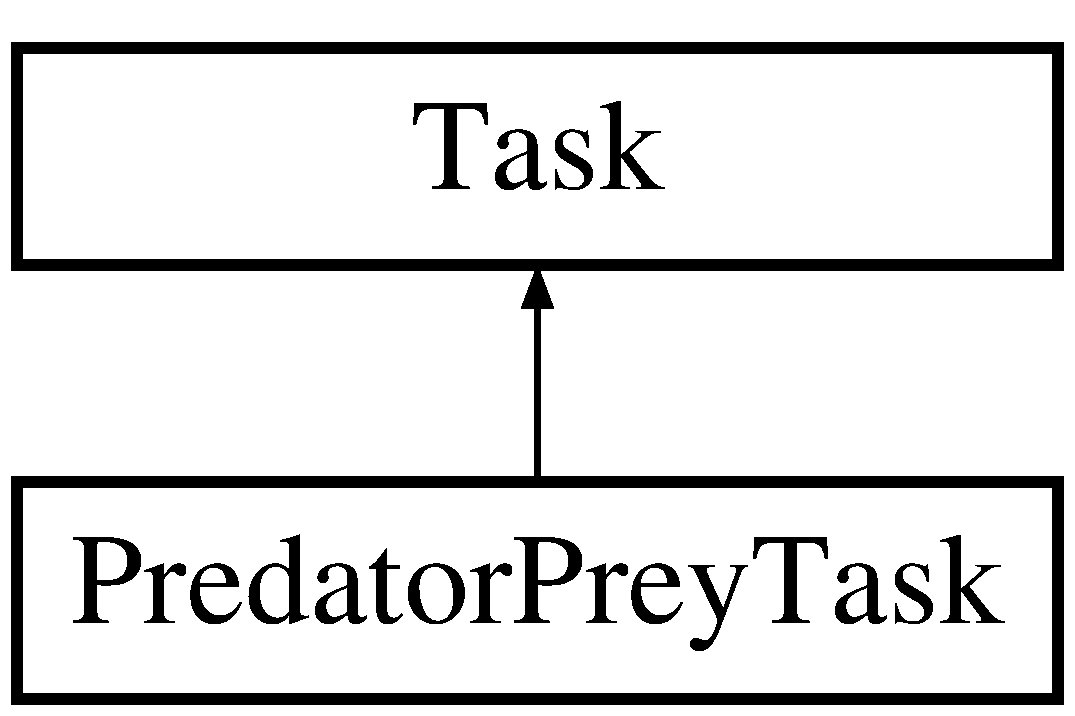
\includegraphics[height=2.000000cm]{a00005}
\end{center}
\end{figure}
\subsection*{Public Member Functions}
\begin{DoxyCompactItemize}
\item 
def {\bf \+\_\+\+\_\+init\+\_\+\+\_\+}\label{a00005_ac775ee34451fdfa742b318538164070e}

\begin{DoxyCompactList}\small\item\em Constructor method. \end{DoxyCompactList}\item 
def {\bf get\+\_\+reward}
\begin{DoxyCompactList}\small\item\em A reward function. \end{DoxyCompactList}\item 
def {\bf refresh\+\_\+state}
\begin{DoxyCompactList}\small\item\em Update current state loading the data from database. \end{DoxyCompactList}\end{DoxyCompactItemize}
\subsection*{Public Attributes}
\begin{DoxyCompactItemize}
\item 
{\bf database}\label{a00005_a64dbaa3229ec575b68ec333442e10cee}

\begin{DoxyCompactList}\small\item\em Handles connection to the Redis database. \end{DoxyCompactList}\item 
{\bf state}\label{a00005_adc6e5733fc3c22f0a7b2914188c49c90}

\begin{DoxyCompactList}\small\item\em Stores current state. \end{DoxyCompactList}\end{DoxyCompactItemize}


\subsection{Detailed Description}
Implementation of Task interface for a so called Predator-\/\+Prey task. 

\subsection{Member Function Documentation}
\index{Predator\+Prey\+Task\+::\+Predator\+Prey\+Task@{Predator\+Prey\+Task\+::\+Predator\+Prey\+Task}!get\+\_\+reward@{get\+\_\+reward}}
\index{get\+\_\+reward@{get\+\_\+reward}!Predator\+Prey\+Task\+::\+Predator\+Prey\+Task@{Predator\+Prey\+Task\+::\+Predator\+Prey\+Task}}
\subsubsection[{get\+\_\+reward}]{\setlength{\rightskip}{0pt plus 5cm}def get\+\_\+reward (
\begin{DoxyParamCaption}
\item[{}]{self, }
\item[{}]{state}
\end{DoxyParamCaption}
)}\label{a00005_aa97b81cdb2e9a08c63eab0ca7e94bf66}


A reward function. 

If agent is closer to target than 0.\+5m cca 0.\+15 normalized and rotated less than 30 degrees, its considered to be a target state so the reward is 0. Else reward is equal 0.\+01 
\begin{DoxyParams}{Parameters}
{\em state} & Current environment state \\
\hline
\end{DoxyParams}
\begin{DoxyReturn}{Returns}
Returns a reward for a give state 
\end{DoxyReturn}
\index{Predator\+Prey\+Task\+::\+Predator\+Prey\+Task@{Predator\+Prey\+Task\+::\+Predator\+Prey\+Task}!refresh\+\_\+state@{refresh\+\_\+state}}
\index{refresh\+\_\+state@{refresh\+\_\+state}!Predator\+Prey\+Task\+::\+Predator\+Prey\+Task@{Predator\+Prey\+Task\+::\+Predator\+Prey\+Task}}
\subsubsection[{refresh\+\_\+state}]{\setlength{\rightskip}{0pt plus 5cm}def refresh\+\_\+state (
\begin{DoxyParamCaption}
\item[{}]{self}
\end{DoxyParamCaption}
)}\label{a00005_a09e7b7d13235130045548d33b3352a1d}


Update current state loading the data from database. 

\begin{DoxyReturn}{Returns}
Returns current environment state 
\end{DoxyReturn}

\section{Task Class Reference}
\label{a00006}\index{Task@{Task}}


Provides a default interface for Tasks used in N\+F\+Q.  


Inheritance diagram for Task\+:\begin{figure}[H]
\begin{center}
\leavevmode
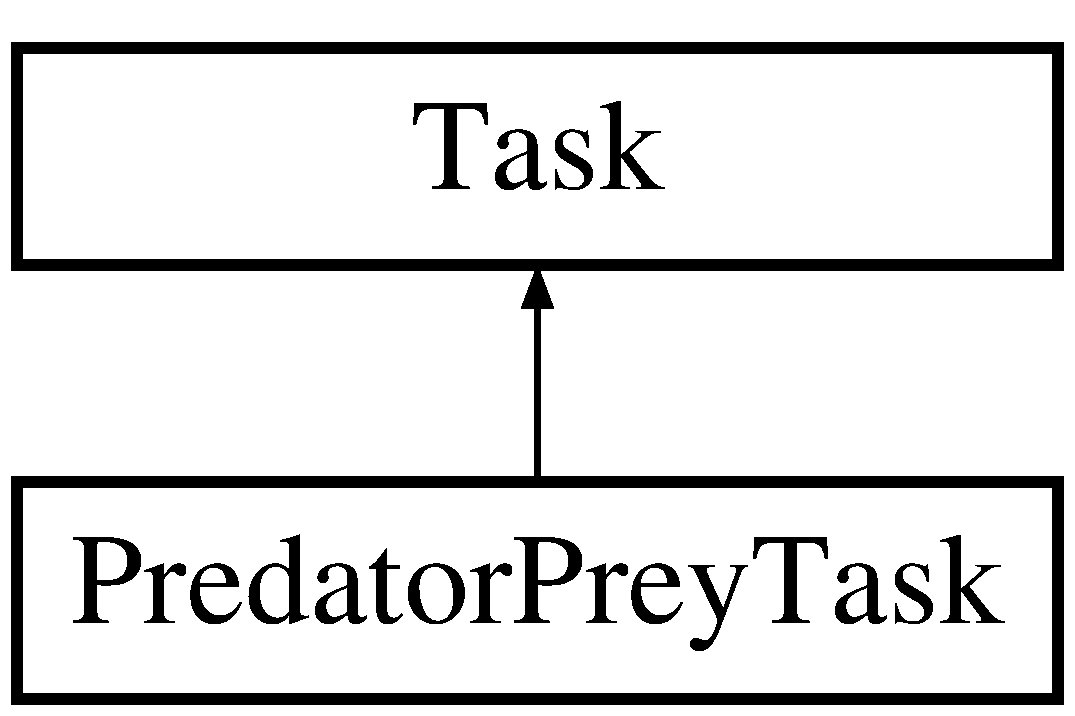
\includegraphics[height=2.000000cm]{a00006}
\end{center}
\end{figure}
\subsection*{Public Member Functions}
\begin{DoxyCompactItemize}
\item 
def {\bf get\+\_\+reward}
\begin{DoxyCompactList}\small\item\em Reward function. \end{DoxyCompactList}\item 
def {\bf refresh\+\_\+state}
\begin{DoxyCompactList}\small\item\em Method for updating environment state. \end{DoxyCompactList}\end{DoxyCompactItemize}


\subsection{Detailed Description}
Provides a default interface for Tasks used in N\+F\+Q. 

\subsection{Member Function Documentation}
\index{Task\+::\+Task@{Task\+::\+Task}!get\+\_\+reward@{get\+\_\+reward}}
\index{get\+\_\+reward@{get\+\_\+reward}!Task\+::\+Task@{Task\+::\+Task}}
\subsubsection[{get\+\_\+reward}]{\setlength{\rightskip}{0pt plus 5cm}def get\+\_\+reward (
\begin{DoxyParamCaption}
\item[{}]{self, }
\item[{}]{state}
\end{DoxyParamCaption}
)}\label{a00006_aa97b81cdb2e9a08c63eab0ca7e94bf66}


Reward function. 

This method has to be implemented \index{Task\+::\+Task@{Task\+::\+Task}!refresh\+\_\+state@{refresh\+\_\+state}}
\index{refresh\+\_\+state@{refresh\+\_\+state}!Task\+::\+Task@{Task\+::\+Task}}
\subsubsection[{refresh\+\_\+state}]{\setlength{\rightskip}{0pt plus 5cm}def refresh\+\_\+state (
\begin{DoxyParamCaption}
\item[{}]{self}
\end{DoxyParamCaption}
)}\label{a00006_a09e7b7d13235130045548d33b3352a1d}


Method for updating environment state. 

This method has to be implemented 
\section{W\+S\+Handler Class Reference}
\label{a00007}\index{W\+S\+Handler@{W\+S\+Handler}}


Handles websocket communication with web app.  




Inherits Web\+Socket\+Handler.

\subsection*{Public Member Functions}
\begin{DoxyCompactItemize}
\item 
def {\bf open}
\begin{DoxyCompactList}\small\item\em Handles all new connections. \end{DoxyCompactList}\item 
def {\bf on\+\_\+message}
\begin{DoxyCompactList}\small\item\em Handles various type of messages received over W\+S. \end{DoxyCompactList}\item 
def {\bf on\+\_\+close}\label{a00007_a278f5ae83d49aaff3f84e571d3af6f47}

\begin{DoxyCompactList}\small\item\em Handles close of W\+S connection from client. \end{DoxyCompactList}\end{DoxyCompactItemize}


\subsection{Detailed Description}
Handles websocket communication with web app. 

\subsection{Member Function Documentation}
\index{server\+::\+W\+S\+Handler@{server\+::\+W\+S\+Handler}!on\+\_\+message@{on\+\_\+message}}
\index{on\+\_\+message@{on\+\_\+message}!server\+::\+W\+S\+Handler@{server\+::\+W\+S\+Handler}}
\subsubsection[{on\+\_\+message}]{\setlength{\rightskip}{0pt plus 5cm}def on\+\_\+message (
\begin{DoxyParamCaption}
\item[{}]{self, }
\item[{}]{json\+\_\+message}
\end{DoxyParamCaption}
)}\label{a00007_a7618f0d180e9433d4fda68fdcc77b883}


Handles various type of messages received over W\+S. 

It distinc 3 main commands\+:
\begin{DoxyItemize}
\item Performing an action.
\item Saving current task.
\item Running loaded task.
\end{DoxyItemize}

It also responds with corresponding data 
\begin{DoxyParams}{Parameters}
{\em json\+\_\+message} & Data received in W\+S request (like action number) \\
\hline
\end{DoxyParams}
\index{server\+::\+W\+S\+Handler@{server\+::\+W\+S\+Handler}!open@{open}}
\index{open@{open}!server\+::\+W\+S\+Handler@{server\+::\+W\+S\+Handler}}
\subsubsection[{open}]{\setlength{\rightskip}{0pt plus 5cm}def open (
\begin{DoxyParamCaption}
\item[{}]{self}
\end{DoxyParamCaption}
)}\label{a00007_ae4b82667a73596ae2d8042e9b4be8a95}


Handles all new connections. 

Initializes a new N\+F\+Q instance for each new W\+S connection 
%--- End generated contents ---

% Index
\newpage
\phantomsection
\addcontentsline{toc}{chapter}{Index}
\printindex

\end{document}
